\section{Details} % Main chapter title
This section is going to describe how the authentication process takes place in detail. The picture below gives a general overview of the process. Each step of the diagram is getting described in detail.\\
\label{Details} % For referencing the chapter elsewhere, use \ref{Chapter1} 
\begin{center}
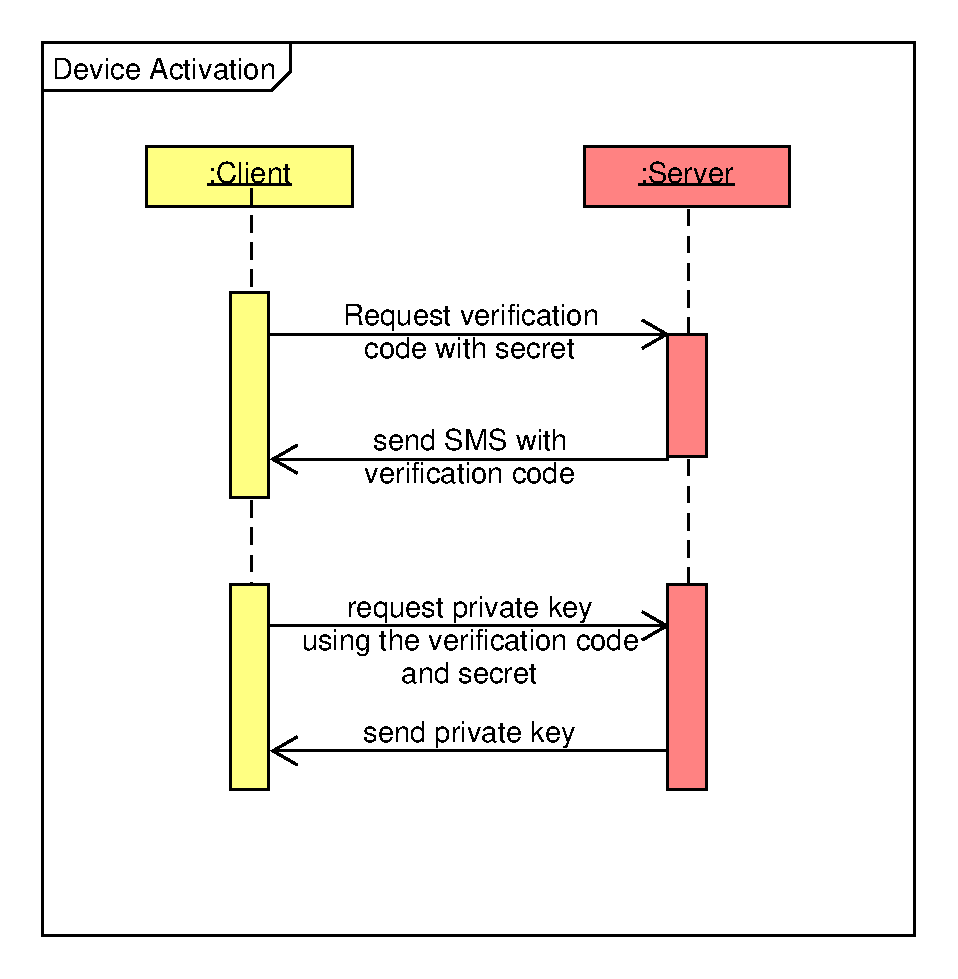
\includegraphics[height=10cm]{figures/deviceactivation.pdf}
\end{center}
\captionof{figure}{Activation of Device}

\subsection{Request Verification Code}
In this step the request to receive a SMS with the verification code is send. The request contains the personal information of the user, the phone number and a secret. If it is not the first time for the user to use this phone number, no personal information needs to be send. The secret is simply a randomly generated 32 characters long string. The use for this string is explained in a later part. In the database a new user is created or updated with the newly given information (phone number, personal information and secret).

\subsection{Send SMS with Verification Code}
Once the backend has processed the previous request, a SMS is send to the given phone number containing a randomly generated six digit number. This number is then stored with a reference to the user in the database.

\subsection{Request Private Key}
A new request is send to the backend containing the six digit verification code and the secret from the first step. Here the secret becomes important. A attacker could have intercepted the SMS and could now validate his device with the verification code, but because he does not know the secret from the first step he can not complete this step. When the verification code request is send SSL encryption is used so the secret can not be read.\\
If the verification code and the secret are the same as in the database this step sends back a private key. This key is then used by the user to make any requests to any resource to the backend and needs to be locally encrypted and stored on the device.

\subsection{Requesting a Resource}
If any resource is requested the private key needs to be provided in the request header in the "X-Auth-Token" field. If the key is missing a response with the code 403 is send.

\begin{center}
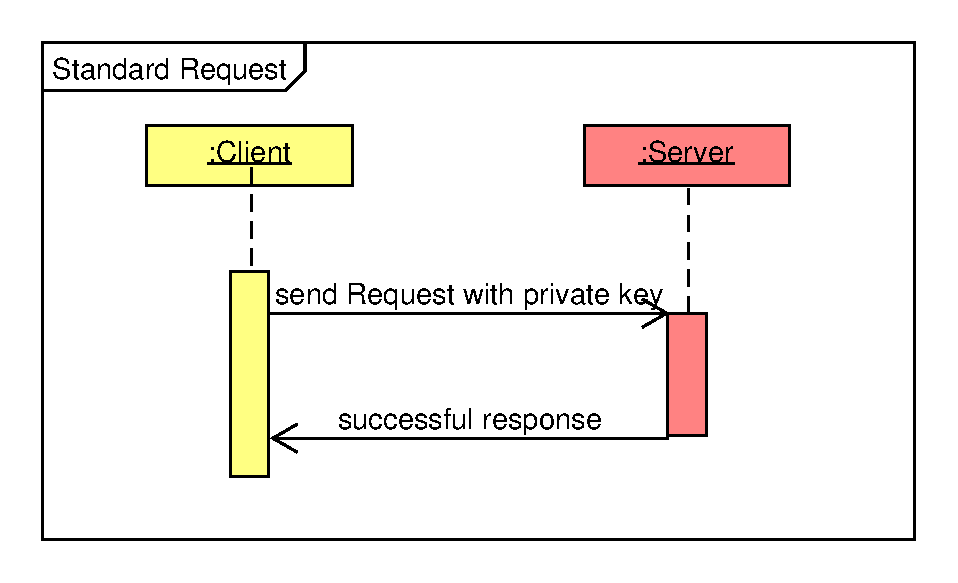
\includegraphics[height=6.6cm]{figures/SuccessfulRequest.pdf}
\end{center}
\captionof{figure}{Valid request}

\begin{center}
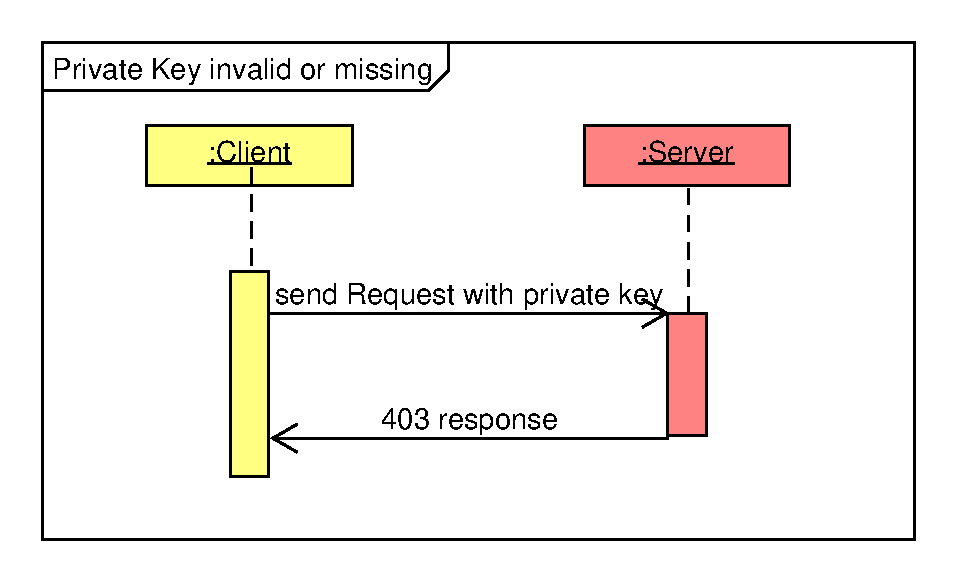
\includegraphics[height=6.6cm]{figures/UnsuccessfulRequest.pdf}
\end{center}
\captionof{figure}{Invalid Request}